\chapter*{人物传记}

\addcontentsline{toc}{chapter}{\protect\numberline{人物传记}{}}
\markboth{人物传记}{人物传记}

\setlength{\parskip}{0.15\baselineskip}

\bigskip

\section*{(一) 康托尔}

\begin{figure}[!h]
\centering
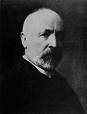
\includegraphics[width=0.3\textwidth]{image/Cantor.jpg}
\\
\centering{康托尔}
\end{figure}

康托尔(1845--1918)德国数学家, 集合论的创始人. 生于俄国圣彼得堡(今俄罗斯列宁格勒), 父亲是犹太血统的丹麦商人, 母亲出身艺术世家. 1856~年全家迁居德国的法兰克福,  先在一所中学, 后在威斯巴登的一所大学预科学校学习. 1862~年入苏黎世大学学工, 翌年转入柏林大学攻读数学和神学, 受教于库默尔、维尔斯特拉斯和克罗内克. 1866~年曾去格丁根学习一学期,  1867~年在库默尔指导下以解决一般整系数不定方程~$ax^2+by^2+cz^2=0$~求解问题的论文获博士学位. 毕业后受维尔斯特拉斯的直接影响, 由数论转向严格的分析理论的研究, 不久崭露头角. 他在哈雷大学任教(1869$\sim$1913年)的初期证明了复合变量函数三角级数展开的唯一性, 继而用有理数列极限定义无理数. 1872~年成为该校副教授, 1879~年任教授. 由于学术观点上受到的沉重打击, 使康托尔曾一度患精神分裂症,  虽在~1887~年恢复了健康, 继续工作, 但晚年一直病魔缠身. 1918~年~1~月~6~日在德国哈雷--维滕贝格大学
附属精神病院去世.

康托尔爱好广泛, 极有个性, 终身信奉宗教. 早期在数学方面的兴趣是数论, 1870~年他开始研究三角级数并由此产生~19~世纪末到~20~世纪初最伟大的数学成就\raisebox{0.5mm}{-----}集合论和超穷数理论的建立. 除此之外,  他还努力探讨在新理论创立过程中所涉及的数理哲学问题.

康托尔对数学的主要贡献是集合论和超穷数理论. 由康托尔首创的全新且具有划时代意义的集合论, 是自古希腊时代的两千多年以来, 人类认识史上第一次给无穷建立起抽象的形式符号系统和确定的运算, 它从本质上揭示了无穷的特性, 使无穷的概念发生了一次革命性的变化, 并渗透到所有的数学分支, 从根本上改造了数学的结构, 促进了数学的其他许多新的分支的建立和发展, 成为实变函数论、代数拓扑、群论和泛函分析等理论的基础, 还给逻辑和哲学带来了深远的影响.

不过康托尔的集合论并不是完美无缺的, 一方面, 康托尔对``连续统假设''和``良序性定理''始终束手无策; 另一方面, 19~和~20~世纪之交发现的布拉利--福蒂悖论、康托尔悖论和罗素悖论, 使人们对集合论的可靠性产生了严重的怀疑. 加之集合论的出现确实冲击了传统的观念, 颠覆了许多前人的想法, 很难为当时的数学家所接受, 遭到了许多人的反对, 其中反对的最激烈的是柏林学派的代表人物之一、构造主义者克罗内克. 克罗内克认为, 数学的对象必须是可构造出来的, 不可用有限步骤构造出来的都是可疑的, 不应作为数学的对象, 他反对无理数和连续函数的理论, 同样严厉批评和恶毒攻击康托尔的无穷集合和超限数理论不是数学而是神秘主义. 他说康托尔的集合论空空洞洞毫无内容,  除了克罗内克之外, 还有一些著名数学家也对集合论发表了反对意见. 法国数学家庞加莱说:``我个人, 而且还不只我一人, 认为重要之点在于, 切勿引进一些不能用有限个文字去完全定义好
的东西''. 他把集合论当作一个有趣的``病理学的情形''来谈, 并且预测说:``后一代将把集合论当作一种疾病
而人们已经从中恢复过来了''. 德国数学家魏尔斯特拉斯认为, 康托尔关于基数的等级观点是``雾上之雾''. 克莱因也不赞成集合论的思想. 数学家施瓦兹原来是康托尔的好友, 但他由于反对集合论而同康托尔断交. 集合论的悖论出现之后, 他们开始认为集合论根本是一种病态, 他们以不同的方式发展为经验主义、
半经验主义、直觉主义、构造主义等学派, 在基础大战中, 构成反康托尔的阵营.
1884~年, 由于连续统假设长期得不到证明, 再加上与克罗内克的尖锐对立, 精神上屡遭打击, 5~月底, 他支持不住了, 第一次精神崩溃. 他的精神沮丧, 不能很好地集中研究集合论, 从此深深地卷入神学、哲学及文学的争论而不能自拔. 不过每当他恢复常态时, 他的思想总变得超乎寻常的清晰, 继续他的集合论的工作.

康托尔的集合论得到公开的承认和热情的称赞应该说首先在瑞士苏黎世召开的第一届国际数学家大会上表现出来. 瑞士苏黎世理工大学教授胡尔维茨在他的综合报告中, 明确地阐述康托尔集合论对函数论的进展所起的巨大推动作用, 这破天荒地向国际数学界显示出了康托尔的集合论
不是可有可无的哲学, 而是真正对数学发展起作用的理论工具. 在分组会上, 法国数学家阿达玛也报告康托尔对他的工作的重要作用. 随着时间的推移, 人们逐渐认识到集合论的重要性. 希尔伯特高度赞誉康托尔的集合论是``数学天才最优秀的作品'', ``人类纯粹智力活动的最高成就之一'', ``这个时代所能夸耀的最巨大的工作''. 在~1900~年第二届国际数学家大会上, 希尔伯特高度评价了康托尔工作的重要性, 并把康托尔的连续统假设
列入~20~世纪初有待解决的~23~个重要数学问题之首. 当康托尔的朴素集合论出现一系列悖论时, 克罗内克的后继者布劳威尔等人借此大做文章, 希尔伯特用坚定的语言向他的同代人宣布:``没有任何人能将我们从康托尔所创造的伊甸园中驱赶出来''.
\bigskip

\section*{(二) 勒贝格}

\begin{figure}[!h]
\centering
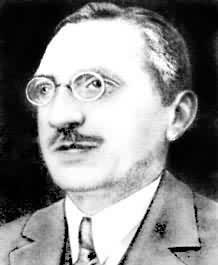
\includegraphics[width=0.3\textwidth]{image/Lebesguetu.jpg}
\\
\centering{勒贝格}
\end{figure}

勒贝格(1875--1941)法国数学家, 生于法国博韦, 父亲是一名印刷厂职工, 酷爱读书, 很有教养. 在父亲的影响下, 勒贝格从小勤奋好学, 成绩优秀, 特别擅长计算. 不幸, 父亲去世过早, 家境衰落. 在学校老师的帮助下进入中学, 后又转学巴黎. 1894~年考入高等师范学校.

1897~年大学毕业后, 勒贝格在该校图书馆工作了两年. 在这期间, 出版了波雷尔关于点集测度的新方法的《函数论讲义》, 特别是研究生贝尔发表了关于不连续实变函数理论的
第一篇论文. 这些成功的研究工作说明在这些崭新的领域中进行开拓将会获得何等重要的成就, 从而激发了勒贝格的热情. 从~1899$\sim$1902~年勒贝格在南锡的一所中学任教, 虽然工作繁忙, 但仍孜孜不倦地研究实变函数理论, 并于~1902~年发表了博士论文``积分、长度、面积'', 在这篇文章中, 勒贝格创立了后来以他的名字命名的积分理论. 此后, 他开始在大学任教(1902$\sim$1906~年在雷恩;1906$\sim$1910~年在普瓦蒂埃), 并出版了一些重要著作:
《积分法和原函数分析的讲义》(1904~年)、《三角级数讲义》(1906~年), 接着, 勒贝格又于~1910$\sim$1919~年在巴黎大学担任讲师, 1920~年转聘为教授, 这时他又陆续发表了许多关于函数的微分、积分理论的研究成果. 勒贝格于~1921~年获得``法兰西学院教授''称号, 翌年作为约当的后继人被选为巴黎科学院院士.

勒贝格对数学的主要贡献属于积分论领域, 这是实变函数理论的中心课题. 19~世纪以来, 微积分开始进入严密化的阶段. 1854~年, 黎曼引入以他的名字命名的积分, 这一理论的应用范围主要是连续函数. 随着维尔斯特拉斯和康托尔工作的问世, 在数学中出现许多``奇怪''的函数与现象, 致使黎曼积分理论暴露出较大的局限性. 几乎与
这一理论发展的同时(1870$\sim$1880~年), 人们就已广泛地开展了对积分理论的改造工作. 当时, 关于积分论的工作主要集中在
无穷集合的性质的探讨, 而无处稠密的集合具有正的外``容度''性质的发现, 使集合的测度概念在积分论的研究中占有重要地位. 积分的几何意义是曲线围成的面积, 黎曼积分的定义是建立在对区间长度的分割的基础上的. 因此, 人们自然会考虑到如何把长度、
面积等概念扩充到更广泛的集合类上, 从而把积分概念置于集合测度理论的框架之中. 这一思想的重要性在于使人们认识到:
集合的测度与可测性的推广将意味着函数的积分与可积性的推广. 勒贝格积分正是建立在勒贝格测度理论的基础上的, 它是黎曼积分的扩充.

为勒贝格积分理论的创立做出重要贡献的首先应推约当, 他在《分析教程》一书中阐述了后人称谓的约当测度论, 并讨论了定义在有界约当可测集上的函数, 采用把区域分割为有限个约当可测集的办法来定义积分. 虽然约当的测度论存在着严重的缺陷(例如存在着不可测的开集, 有理数集不可测等), 而且积分理论也并没有做出
实质性的推广, 但这一工作极大地影响着勒贝格研究的视野. 在这一方向上迈出第二步的杰出人物是波雷尔, 1898~年在他的《函数论讲义》中向人们展示了``波雷尔集''的理论. 他从~$\R$~中的开集是构成区间的
长度总和出发, 允许对可列个开集作并与补的运算, 构成了所谓以波雷尔可测集为元素的~$\sigma$-代数类, 并在其上定义了测度. 这一成果的要点是使测度具备完全可加性(约当测度只具备有限可加性), 即对一列互不相交
的波雷尔集~$\{E_n\}$, 若其并集是有界的, 则其并集的测度等于每个~$E_n$~的测度的和. 此外, 他还指出:集合的测度和可测性是两个不同的概念. 但在波雷尔的测度思想中, 却存在着不是波雷尔集的约当可测集(这一点很可能是使他没有进一步开创积分理论的原因之一). 特别是其中存在着零测度的稠密集, 引起了一些数学家的反感. 然而勒贝格却洞察了这一思想的深刻意义并接受了它. 他突破了约当对集合测度的定义中所作的有限覆盖的限制, 以更加一般的形式发展和完善了波雷尔的测度观念, 给出了集合测度的分析定义:

设~$E \subset [a,\,b]$, 考虑可数多个区间~$\{I_i\}$~对~$E$~作覆盖. 定义数值
\[
m^*(E)=\inf\Big\{ \mathop{\textstyle{\sum}}_i \big| I_i \big|: \: \medcup_i I_i \supset E \Big\}
\]
为勒贝格外测度, 且若
\[
m^*(E) + m^*\big( [a,\,b]-E \big) = b-a
\]
则称~$E$~为可测集(即~$E$~是勒贝格可测的).

在此基础上, 勒贝格引入了新的积分定义:

对于一个定义在~$[a,\,b]$~上的有界实值函数~$f(x)~(M_1 \leqslant f(x) \leqslant M_2)$, 作~$[M_1,\,M_2]$~的分割~$\delta$
\[
M_1 = y_0 < y_1 < \cdots < y_{n-1} < y_n = M_2
\]
令
\[
E_i = \big\{x \in [a,\,b]: \: y_{i-1} \leqslant f(x) \leqslant y_i \big\}, \quad i=1,\,\cdots,\,n
\]
并假定这些集合是可测的(即~$f(x)$~是勒贝格可测函数), 并用~$m(E_i)$~表示~$E_i$~的
勒贝格测度. 考虑和式
\[
s_\delta = \sum_{i=1}^n y_{i-1} \cdot m(E_i), \quad S_\delta = \sum_{i=1}^n y_i \cdot m(E_i)
\]
如果当~$\max\{y_i - y_{i-1}\} \to 0$~时, $s_\delta$~与~$S_\delta$~趋于同一极限值, 则称此值为~$f(x)$~在~$[a,\,b]$~上的积分.

勒贝格曾对他的这一积分思想做过一个生动有趣的描述:

\begin{quote}
``我必须偿还一笔钱. 如果我从口袋中随意地摸出来各种不同面值的钞票, 逐一地还给债主直到全部还清, 这就是黎曼积分;不过, 我还有另一种做法, 就是把钱全部拿出来并把相同面值的钞票放在一起, 然后再一起付给应还的数目, 这就是我的积分.''
\end{quote}


从他的这一新思想中, 任何约当可测集、波雷尔可测集都是勒贝格可测集. 勒贝格积分的范围包括了由贝尔引入的一切不连续函数.

从数学发展的历史角度看, 新的积分理论的建立是水到渠成的事情. 但是可贵的是, 与同时代的一些数学家不同, 在勒贝格看来, 积分定义的推广只是他对积分理论研究的出发点, 他深刻的认识到, 在这一理论中蕴含着一种新的
分析工具, 使人们能在相当大范围内克服黎曼积分中产生的许多理论困难. 而这些困难所引起的问题正是促使
勒贝格获得这一巨大成就的动力.

这方面的第一个问题是早在~19~世纪初期由傅里叶在关于三角级数的工作中不自觉地引发的: 当一个有界函数可以表示为一个三角级数时, 该级数是它的
傅里叶级数吗？这一问题与一个无穷级数是否可以逐项积分有着密切的关系. 傅里叶当时曾认为在其和为有界函数时
这一运算是正确的, 从而给上述问题以肯定的回答. 然而到了~19~世纪末期, 人们认识到逐项积分并不总是可行的, 甚至对于黎曼可积函数的一致有界的级数也是这样, 因为由该级数所表示的函数不一定是黎曼可积的. 这个问题的讨论
促使勒贝格在新的积分理论中获得了一个十分重要的结果\raisebox{0.5mm}{-----}控制收敛定理. 作为一个特殊情形他指出, 勒贝格可积的
一致有界级数都可以逐项进行积分, 从而支持了傅里叶的结论. 逐项积分在本质上就是积分号下取极限的问题, 它是积分论中经常遇到的最重要的运算之一. 从而这一定理的创立显示出勒贝格积分理论的极大优越性.

微积分基本公式
\[
\int_a^x f'(x) \mathrm{d} x = f(x)-f(a), \quad x \in [a,\,b]
\]
是微积分学的核心. 然而这一公式的运用在黎曼积分意义下却有较大的局限性. 在~1878$\sim$1881~年间, 迪尼和沃尔泰拉曾构造了这样的函数, 它们具有有界的导函数, 但是导函数不是黎曼可积的, 从而基本定理
对此是不适用的. 此后, 联系到黎曼积分对无界函数的推广也发现了类似的困难. 然而, 在新的积分理论中, 勒贝格指出, 对有界函数来说, 这一困难是不存在的. 在~$f'(x)$~是有限值但无界的情形, 只要是可积的, 基本定理仍是成立的, 而且这正相当于~$f(x)$~是有界变差函数. 同时, 逆向问题也被人们提出来了:
何时一个连续函数是某个函数的积分？为此, 哈纳克曾导入了后来叫作绝对连续的函数. 约在~1890~年期间, 绝对连续函数就被当作绝对收敛的积分
的特征性质来研究, 虽然还没有人能真正证明任何绝对连续函数都是一个积分. 然而, 勒贝格通过对于导数
几乎处处为零但函数本身并非常数的函数的考察, 认识到在他的积分意义下, 上述结论是正确的. 从而得出了积分与原函数之间的一个完整结果: 微积分基本公式成立的充要条件是, $f(x)$~是~$[a,\,b]$~
上的绝对连续函数.

另一个与积分论有关的问题是曲线的长度问题. 19~世纪前期, 很少有人注意到一条曲线长度的定义和可求长问题. 一般都认为以~$y=f(x)~(a \leqslant x \leqslant b)$~所描述的曲线段总是有长度的, 且长度可用
\[
L=\int_a^b \big[ 1+[f'(x)]^2 \big]^\frac{1}{2} \mathrm{d} x
\]
表示. 杜布瓦雷蒙在研究关于两点间长度最短的曲线的变分问题时, 从狄利克雷关于函数的一般观点出发探讨了曲线长度的概念. 由于用到了极限过程这一分析手段, 他认为积分理论对曲线长度的概念和可求长性质的陈述是必不可少的. 而到了~19~世纪末期, 这一见解由于希弗尔举出了反例而更为尖锐, 这一反例致使定积分
\[
\int_{x_0}^{x_1} \big[ 1+[f'(x)]^2 \big]^\frac{1}{2} \mathrm{d} x
\]
在黎曼积分的定义下没有意义. 勒贝格对这一问题很感兴趣, 并应用他的积分理论中的方法和结果, 证明了曲线长度与积分概念是密切相关的, 从而恢复了杜布瓦雷蒙断言的可信性.

勒贝格关于微积分基本公式和曲线可求长理论的研究, 促使他发现有界变差函数是几乎处处可微的这一事实.
%\footnote{约当曾指出不定积分是有界变差函数. }% 
这一定理的重要性在于: 人们对连续函数的可微性已经讨论
了一个多世纪, 在~19~世纪的几乎前半个世纪, 人们还一直认为连续函数在其定义区域中绝大多数点上都是
可微的. 虽然连续函数总被误认为是逐段单调的, 但这使单调性与可微性联系起来了, 尽管是脆弱的. 到~19~世纪末期, 这一看法逐渐被人怀疑, 甚至有些其地位不低于维尔斯特拉斯的数学家都觉得存在这无处可微的连续的单调函数. 于是, 在这一意义下, 勒贝格的定理支持了老一代数学家的直觉印象.

在传统的关于二重积分与累次积分的恒等性定理上, 黎曼积分也反映出它的不足之处, 人们发现了使该定理不成立的
例子. 而作为一个结论, 这一定理的传统说法必须修改, 然而在把积分推广到无界函数的情形时, 这一修改变得更加严峻. 对此, 勒贝格的重积分理论, 使得用累次积分来计算二重积分的函数范围扩大了. 他在~1902~年给出的一个结果奠定了~1907~年富比尼创立的著名定理的基础.

\setcounter{footnote}{0}

勒贝格积分理论作为分析学中的一个有效工具的出现, 尤其是他在三角级数中应用的高度成功, 吸引了许多数学家的兴趣. 例如法都、里斯、费舍尔等都来探讨有关的问题, 使这一领域开始迅速发展, 其中特别是里斯关于~$L^p$~空间的工作\footnote{勒贝格可积函数的全体
构成的距离空间是完备的. }, 使得勒贝格积分在积分方程和函数空间的理论中持久地占有重要的位置.

虽然勒贝格在最初阶段专注于他自己的积分理论, 然而在激励抽象测度和积分论研究的开展上, 他的工作仍是先导性的. 1910~年, 勒贝格发表题为~``关于不连续函数的积分''的重要专题报告. 在这里他不仅把积分、微分理论推广到~$n$~维空间, 而且引入了可数可加集合函数的概念(定义在勒贝格可测集类上), 指出这些函数是定义在集合类上的有界变差函数. 正是因为对于
有界变差与可加性概念之间联系的考察, 使得拉东作出了更广的积分定义, 其中把斯蒂尔杰斯积分和勒贝格积分作为它的特殊情形. 他还在~1913~年的文章中指出, 勒贝格的思想在更一般的背景上也是有效的.

勒贝格的一生都献给了数学事业. 1922~年被推举为院士时, 他的著作和论文已达~90~多种之多, 内容除积分理论外, 还涉及集合与函数的构造\footnote{后来由苏联数学家卢津及其他学者进一步做出发展. }、变分法、曲面面积以及维数理论等重要课题. 在勒贝格生前最后~20~年, 研究工作仍然十分活跃并反映出广泛的兴趣, 不过作品内容大都涉及教育、历史等.

勒贝格的工作是对本世纪科学领域的一个重大贡献, 但和科学史上所有新思想运动一样, 并不是没有遇到阻力的. 原因是在勒贝格的研究中扮演了重要角色的那些不连续函数和不可微函数被人认为违反了所谓的完美性法则, 是数学中的变态和不健康部分. 因此, 他的工作受到了某些数学家的漠视, 甚至有人曾企图阻止他关于一篇讨论不可微曲面的论文的发表. 勒贝格曾感叹地说:``我被称为是一个没有导数的函数的那种人了！''
然而, 不论人们的主观愿望如何, 这些具有种种奇异性质的对象都自动地进入了研究者曾企图避开它们的问题之中. 勒贝格充满信心地指出:``使得自己在这种研究中变得迟钝了的那些人, 是在浪费他们的时间, 而不是在从事有用的工作. ''

由于在实变函数理论方面的杰出成就, 勒贝格相继获得胡勒维格奖(1912~年);
彭赛列奖(1914~年)和赛恩吐奖(1917~年). 许多国家和地区(如伦敦、罗马、丹麦、
比利时、罗马尼亚和波兰)的科学院都聘他为院士, 许多大学授予他名誉学位, 以表彰他的贡献.

\bigskip

\section*{(三) 黎曼}

\begin{figure}[!h]
\centering
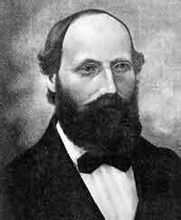
\includegraphics[width=0.3\textwidth]{image/Riemanntu.jpg}
\\
\centering{黎曼}
\end{figure}

1826~年~9月~17~日, 在德国汉诺威的布列斯伦茨, 黎曼(1826--1866)出生在一个乡下牧师之家, 是六个孩子中的次子. 黎曼从小酷爱数学. 他~6~岁时开始学习算术, 并显现出他的数学天才. 他不仅能解决所有留给他的数学问题, 而且还经常提一些问题来捉弄他的兄弟姐妹. 10~岁时他跟一位职业教师学习高级算数和几何, 很快便超过了老师, 常常对一些问题能做出更好的答案.

黎曼~14~岁时到汉诺威市上中学. 由于经济拮据, 他总是靠步行奔波于汉诺威市与乡间小村庄之间. 当然他更没钱去买参考书. 幸运的是中学校长及时地发现了他的数学才能, 考虑到他经济上的困难, 校长特许黎曼可以从自己私人藏书室里借阅数学书籍. 在校长的
推荐下, 黎曼借了一部数学家勒让德的《数论》, 这是一部共~859~页的四大本的名著. 黎曼十分珍惜这种读书机会, 他如饥似渴地自学起来, 六天之后, 黎曼便学完并归还了这本书. 校长问他:``你读了多少？''黎曼说:``这是一本了不起的书, 我已经掌握了它. ''几个月之后, 校长就这本书的内容考他, 黎曼对答如流, 并且回答得很全面. 利用校长的藏书, 黎曼还抓紧时间很快地
自学了大数学家欧拉的著作, 由此掌握了微积分及其分支. 黎曼
不仅从欧拉的著作中学到了数学知识, 还学到了欧拉研究数学的技巧.

19~岁时, 黎曼进入格丁根大学学习, 为了在经济上帮助家庭以尽快找到一个有报酬的
工作, 他先攻读哲学和神学. 但是, 除了这两门课程以外, 他也去听数学、物理学课程. 他听了斯特恩关于方程论和定积分、高斯关于最小二乘法以及戈尔德斯米特关于地磁学的
数学讲座, 对数学专业产生了难以割舍的兴趣.

黎曼向父亲讲述了这一切, 请求允许自己改学数学专业. 父亲由衷地同意了他的请求. 黎曼极为高兴, 并深深地感激父亲. 1847~年, 为了师从更多的大师, 黎曼转学到柏林大学, 就学于大数学家雅可比、
狄利克雷、斯泰纳和艾森斯坦门下. 他从雅可比那里学到高等力学和高等代数, 从狄利克雷那
里学到数论和分析学, 从斯泰纳那里学到现代几何, 从艾森斯坦那里学到椭圆函数论. 在此期间, 他极为勤奋, 甚至放假期间也不休息. 1847~年秋假, 黎曼找到几份巴黎科
学院《院刊》, 上面载有数学家柯西新发表的关于单复变量解析函数的论文, 他一眼便看
出这是一种新数学理论, 于是一连几个星期闭门不出, 潜心研究柯西的论文, 并酝酿出他
在这个专题上的新见解, 为四年后撰写博士论文``单复变量函数的一般理论的基础''奠定了
基础.

黎曼不仅认真研读大师的学术专著, 而且虚心地向大师求教. 有一次, 狄利克雷来格
丁根度假, 黎曼趁此机会向他求教数学问题, 并将自己未定稿论文交给他, 请他提意见. 狄利克雷被黎曼的谦虚、真诚和天才迷住了. 他与黎曼长谈了两个小时, 给黎曼的论文提
了不少意见, 给黎曼正在研究的课题作了许多指点, 黎曼深感受益匪浅, 他说没有狄利克
雷的指点, 他将不得不在图书馆里做好几天的吃力研究. 生活虽然清贫, 但学习极为勤勉, 这使得黎曼在大学毕业时获得了丰硕的成果. 1851~年底, 黎曼将其博士论文呈交给大数学家高斯审阅. 高斯在看了论文之后兴奋不已, 对黎曼的论文做出了高度评价, 这对高斯来说是罕见的. 高斯评语道:``黎曼先生交来的论文提供了令人信服的证据, 说明作者对该文所论述的这一问题做了
全面深入的研究, 说明作者具有创造性的、活跃的、真正的数学头脑, 具有灿烂丰富的创造力. ''

1852~年初, 黎曼凭借优异的学术表现取得了博士学位, 并留在了格丁根大学. 19~世
纪中叶的德国, 科学几乎与国家的经济全然无关. 大学的设立仅在训练律师、医师、教师
和传教士, 以及提供贵族子弟和富家子弟度过引人侧目及受尊敬的岁月的场所. 只有正
教授才可以领政府的津贴, 并且可以教正规标准课程, 这些课程都是一些基础科目.上课
的学生多, 因此教授收到的学费也就多了, 这就是为什么当时课程水准低落的原因, 因为
如果课程太难, 就没有办法收到许多学生, 从而影响到教授们的收入, 毕竟贵族子弟和富
家子弟上大学的目的并非真心向学. 讲师们则没有政府津贴并且轮不到教基本正规课程的
机会, 全然靠来听课的学生的学费维生, 通常, 听课的学生不会多, 因此收入也就相当微
薄, 生活非常困苦. 担任讲师是成为正教授的必经途径, 但是却没有明文规定什么时候能
将一位讲师升级为教授, 为了照顾特別值得重视的学者而却没有正教授的空缺时, 政府可
任命他为``客座教授'', 使他具有教基本正规课程的资格, 增多他的收入, 但是这个任命
附有条件, 言明政府不付任何津贴. 因此, 在担任讲师期间, 黎曼没有任何自主的生活费
来源, 生活依旧贫穷. 但黎曼不顾生活上的贫困, 仍然把全部精力投向数学. 他认为只要
能够勉强维持生活, 能够让他研究数学, 他就心满意足了. 他从不因经济上的拮据而感到沮丧. 他一方面积极准备``无薪讲师''的就职演讲论文, 另一方面认真从事数学物理方面的研究工作. 他的
就职论文具有相当的难度. 当初为了确定论文的选题, 他向高斯提交了~3~个题目, 以便让高
斯在其中选定一个. 其中第~3~个题目是涉及几何基础的, 这个题目黎曼当时并没有多少案头
准备工作, 因此黎曼从心底里希望高斯不要选中它. 可是, 高斯对第~3~个题目却深有研究, 他已思考这个问题达~60~年之久. 出于想看看黎曼对这个深奥的问题会做些什么样的创造性
工作, 高斯指定第~3~个题目作为黎曼就职演讲论文的题目. 事后, 黎曼在向父亲谈起这件事
时说, ``所以我又处在绝境中了'', ``我不得不做出这个题目''.

对数学物理研究, 黎曼也具有无限的热情, 他当时曾对人说:``我对于把一切与物理
规律结合起来的数学研究非常入迷. ''``我通过对电、光、磁等之间联系的总研究, 发现
了对这个现象的解释. 这件事对我很重要, 因为这是我第一次能够把我的工作应用到未知
的现象上. ''这两项研究在当时都是高水平的, 因而也是极困难的. 黎曼不顾生活清贫、
营养不良, 超负荷地忘我工作, 长时期过度紧张地思索, 以致他常常体力衰竭, 甚至
病倒. 一旦身体稍有复原, 他又继续研究. 功夫不负有心人, 1854~年~6~月~10~日, 黎曼以``关
于构成几何基础的假设''论文做了就职演讲, 受到了与会数学家们的认可和好评. 高斯听
完之后大为惊异, 感到这个年轻人处理这个难题非常之好, 他赞不绝口. 黎曼的这篇论文
被人们认为是~19~世纪数学史上的杰作之一.

1855~年格丁根大学开始给黎曼发薪金, 但相当的低, 一年仅相当于~200~美元. 这一年黎
曼~29~岁, 他家里遭到巨大的不幸, 父亲和一个妹妹相继去世, 原来依靠父亲生活的~3~个妹妹
失去了生活来源. 于是黎曼和他的哥哥两人挑起了照顾~3~个妹妹生活的担子, 黎曼时时为一
家人的生活感到焦虑. 1857~年黎曼一年的薪金被加到相当于~300~美元的水平. 由于收入不多, 又要照顾~3~个妹妹, 生活担子重, 黎曼连自己的婚姻大事都不敢考虑. 然而就在这一年, 不幸又从天而降, 黎曼的哥哥又去世了, 这对黎曼来说如同雪上加霜, 照料~3~个妹妹生活的
担子全部落在他一人的肩上. 从~1855~年到~1859~年这~5~年中, 经济拮据、生活清贫一直困绕着
黎曼, 有时一家甚至陷入对口粮都需要算计的地步. 就是在这种情况下, 黎曼仍不顾物质
生活的贫乏, 全身心地投入到数学研究工作之中, 在科学的崎岖小道上艰苦奋斗, 并获得
了令人惊异的成就. 他在数学上的许多重要成果都是在这个时期内完成的. 他对阿贝尔积
分和阿贝尔函数的研究, 开创了现代代数几何;他首创用复解析函数研究数论问题, 开创
了现代意义的解析数论;他对超几何级数的研究, 推动了数学物理和微分方程理论的发展. 随着研究成果的问世, 黎曼在数学界的学术声望迅速提高. 他受到许多世界著名数学家
的赞扬, 获得了一个科学家通常可能得到的最高荣誉.

1859~年黎曼~33~岁时, 高斯去世, 他被任命为格丁根大学正教授, 成为继狄利克雷之后
高斯的第二个继任者. 这时黎曼的生活才开始得到改善, 才开始考虑个人的婚姻问题, 并
在~36~岁时与朋友的妹妹结了婚, 一年后, 他的女儿出生在比萨. 但是, 长时期清贫的生活、
过度的操劳、发奋的研究, 使得黎曼身体虚弱、精力衰竭. 1862~年黎曼患了胸膜炎, 不久又患了肺病, 
一年后又患了黄疽病. 在病魔缠身之际, 只
要有一些力气, 黎曼仍坚持数学研究工作. 虽然这个时期黎曼积极就医和疗养, 但因病入
膏盲终无疗效, 1866~年~7~月~20~日, 黎曼那颗纯洁、高尚的心停止了跳动, 他过早地离开了人
世, 也过早地离开了数学, 终年仅~40~岁.

黎曼是数学史上最具独创性精神的数学家之一, 他在众多的数学领域里做出了许多奠
基性和创造性的研究工作\raisebox{0.5mm}{-----}他从几何方向开创了复变函数论;是现代意义的解析数论的奠
基者;他亲手建立了黎曼几何, 是组合拓扑学的开拓者;他对微积分的严格处理作出了重
要贡献;在数学物理和微分方程等领域内也成果丰硕. 1859~年, 黎曼被选为柏林科学院通
讯院士, 1866~年他被选为法国巴黎科学院通讯院士和英国皇家学会国外会员.

%%%%%%%%%%%%%%%%%%%%%%%%%%%%%%%%%%%%%Fubini%%%%%%%%%%%%%%%%%%%%%%%%%%%%%%%%%%%%%%%%%
%\bigskip
%
%\section*{4. 富比尼(Fubini)}
%
%\begin{figure}[!h]
%\centering
%
\includegraphics[width=0.3\textwidth]{images/Fubini.jpg}
%\caption{富比尼(Fubini)}
%\end{figure}
%
%富比尼(G. Fubini, 1879-1943)意大利数学家, 最著名是他的富比尼定理. 富比尼生于威尼斯,
% 早年即因他的老师们和他作数学老师的父亲影响而醉心数学. %1896~年他进了~Scuola Normale Superiore di Pisa, 跟随著名数学家乌利塞·迪尼和路易吉·比安基学习. 他早时已经名声鹊起, 1900~年发表的博士论文《椭圆空间中的克利福德平行》, %在比安基广泛流传的微分几何著作中作了讨论. %
%他获得博士后, 开始担任一连串的教授职位. 1901~年他在西西里的卡塔尼亚大学开始教学, 不久后转到热那亚大学; 1908~年转到都灵的~Politecnico, 接着在都灵大学, 他留在这里数十年. %他这时的研究主要在数学分析, 特别是微分方程、泛函分析和复分析; 但他也研究了变分学、群论、非欧几里得几何和射影几何等学科. %第一次世界大战开始, 他转为从事应用层面的工作, 研究发射炮弹的准确度; 战后他的研究依然朝向应用, 工作成果应用到电路和声学问题. 1939~年, 富比尼年已六旬, 将近退休时, 贝尼托·墨索里尼的法西斯党采取阿道夫·希特勒的纳粹党鼓吹了数年的
%反犹太政策. 身为犹太人, 富比尼担心家庭的安全, 所以应邀到普林斯顿大学任教, 4~年后于纽约市逝世.